\documentclass[12pt]{article}

\usepackage{enumitem}
\usepackage{amsmath}
\usepackage{graphicx}
\usepackage[margin=1in]{geometry}

\title{ECE 442 Notes}
\author{Anthony Jerez}

\begin{document}
    \maketitle
    \setlength{\parindent}{0pt}

    \section{MOSFET Review}

    \subsection*{Device Structure}

    \begin{center}
        \centerline{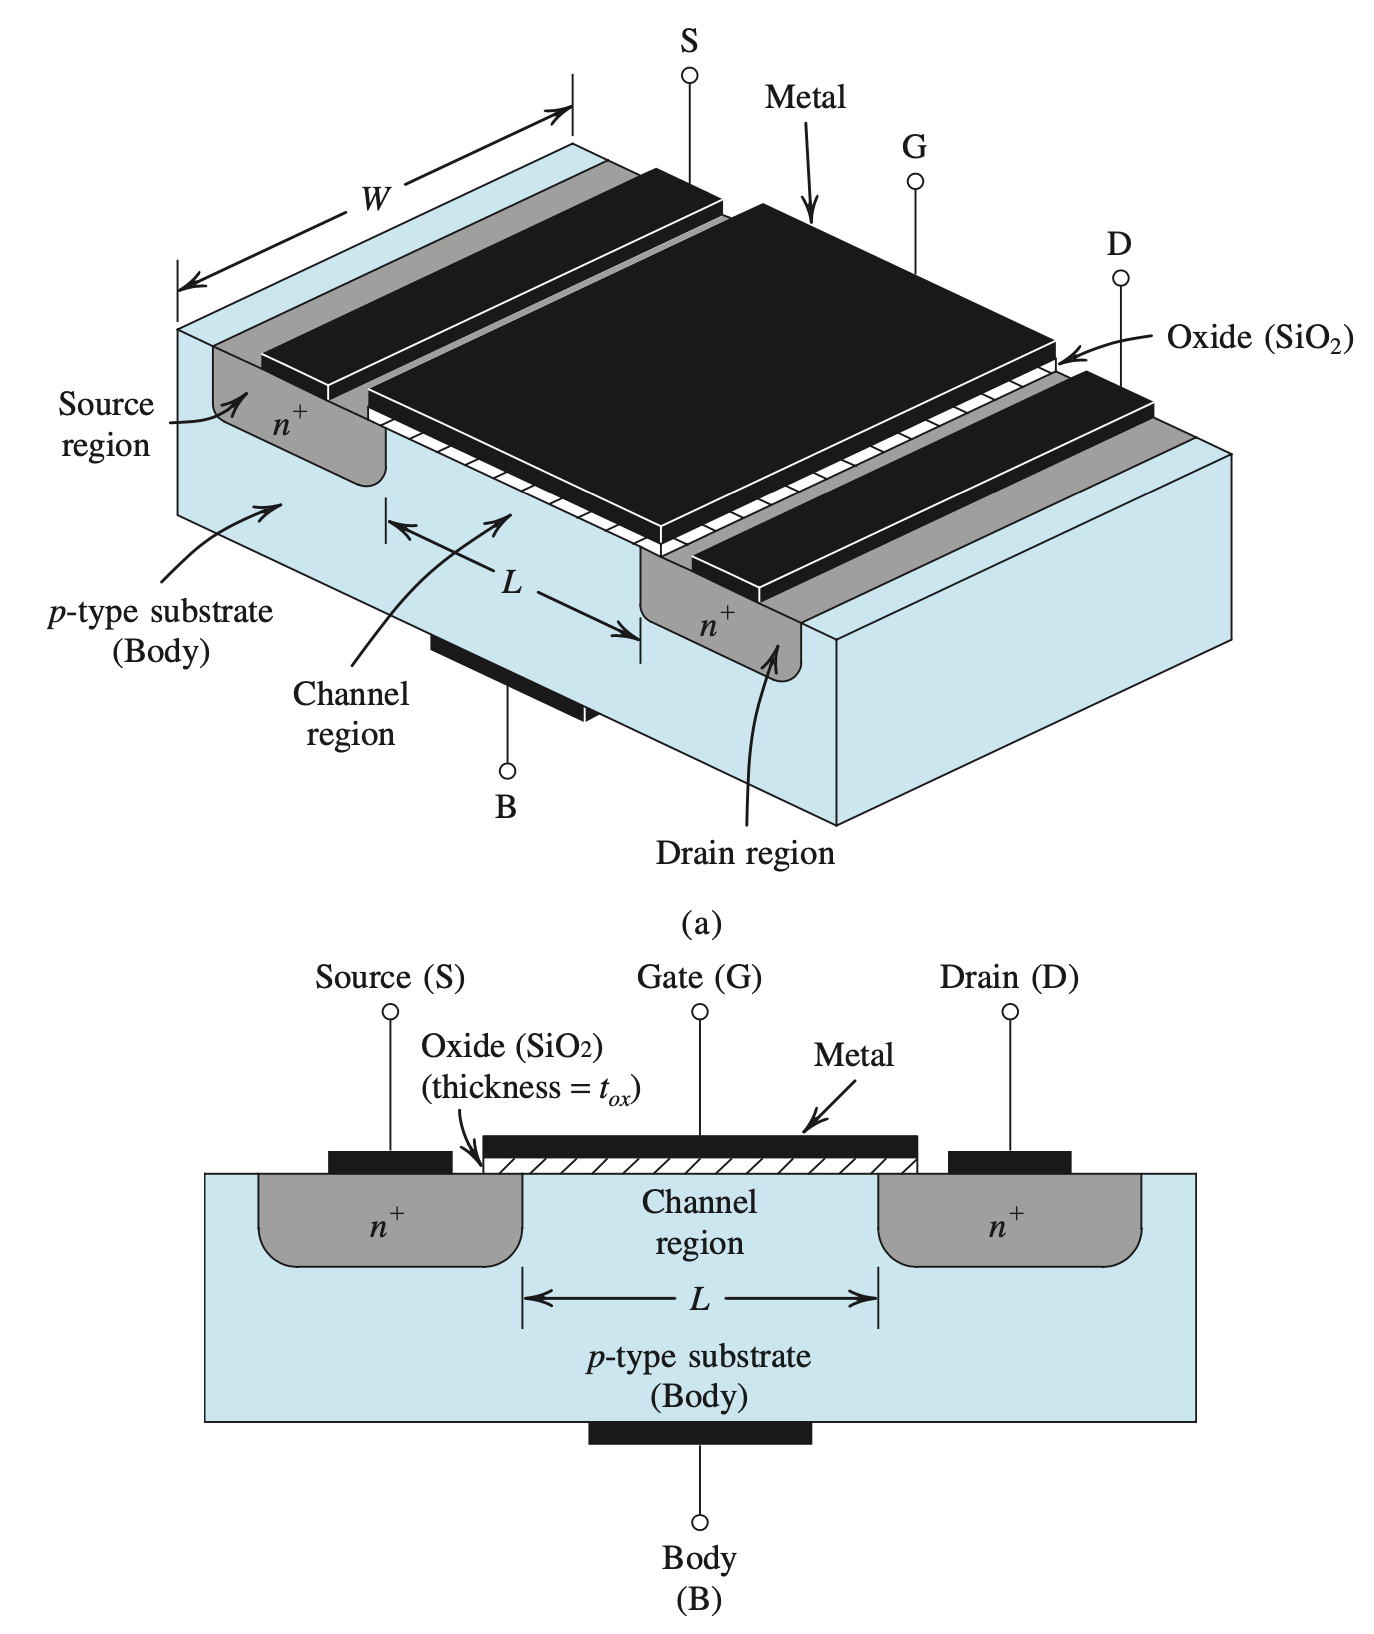
\includegraphics[scale=0.4]{figures/mosfet.png}}
        \textbf{Figure 1.1} Enhancement type NMOS transistor.
    \end{center}

    The voltage applied to the gate controls current flow between the source
    and the drain. This current will flow in the longitudinal direction from 
    the drain to source in the region labeled “channel region."

    \subsection*{Operation with Zero Gate Voltage}

    With zero voltage applied to the gate, two back-to-back diodes exist 
    in series between drain and source. These back-to-back diodes prevent 
    current conduction from drain to source when a voltage $v_{DS}$ is applied. 
    In fact, the path between drain and source has a very high resistance 
    (of the order of $10^{12} \Omega$).

    \subsection*{Creating a Channel for Current Flow}

    Here, both the drain and source are grounded and a positive voltage 
    is applied to the gate. The holes are pushed down into the substrate. The
    posistive gate voltage also attracts electrons from both \textit{n} 
    regions into the channel region. If a voltage is to be applied between 
    the drain and source, current will flow through the \textit{n} region.
    
    \begin{center}
        \centerline{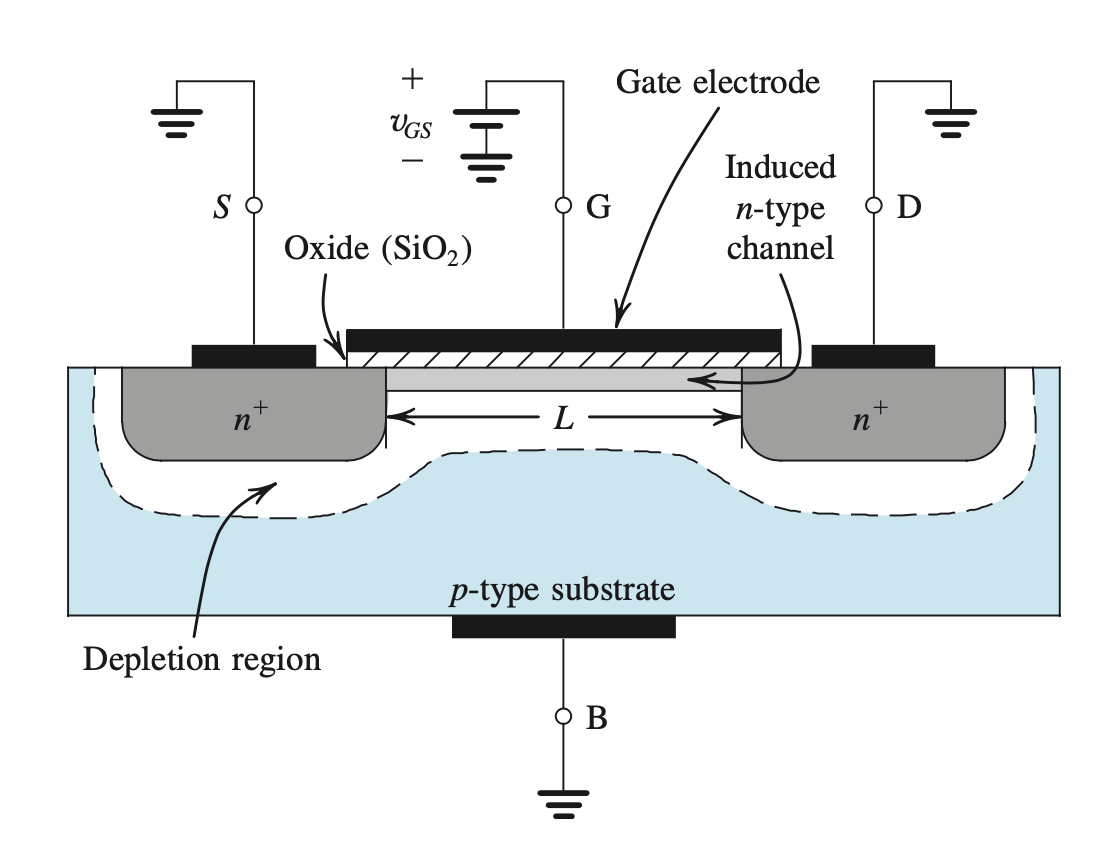
\includegraphics[scale=0.5]{figures/mosfet_induced.png}}
        \textbf{Figure 1.2}
    \end{center}

    A positive voltage applied to the gate causes an abundance of electrons to form near the surface 
    of the substrate under the gate, creating an \textit{n} region.\\[\baselineskip]
    The value of $v_{GS}$ at which a sufficient number of mobile electrons 
    accumulate in the channel region to form a conducting channel is called 
    the threshold voltage and is denoted $V_t$\\
    When $v_{DS} = 0$, the voltage at every point along the channel is zero, 
    and the voltage across the oxide (i.e., between the gate and the points along 
    the channel) is uniform and equal to $v_{GS}$. The excess of $v_{GS}$ over $V_t$ is
    termed the \textit{\textbf{effective voltage}} or the \textit{\textbf{overdrive voltage}} 
    and is the quantity that determines the charge in the channel.
    \begin{align}
        v_{OV} = v_{GS} - V_t
    \end{align}

    We can express the magnitude of the electron charge in the channel by:
    \begin{align}
        |Q| = C_{ox}(WL)v_{OV}
    \end{align}

    where $C_{ox}$, called the \textit{\textbf{oxide capacitance}}, is the capacitance of the 
    parallel-plate capacitor per unit gate area (in units of F/$m^2$), W is the width of the channel, 
    and L is the length of the channel. The oxide capacitance $C_{ox}$ is given by
    \begin{align}
        C_{ox} = \frac{\epsilon_{ox}}{t_{ox}}
    \end{align}

    Finally note that as $v_{OV}$ is increased, the magnitude of the channel charge is 
    increased proportionately. Meaning, the larger the overdrive voltage, the
    deeper the channel.

    \subsection*{Applying a Small $v_{DS}$ (Triode Region)}

    \begin{center}
        \centerline{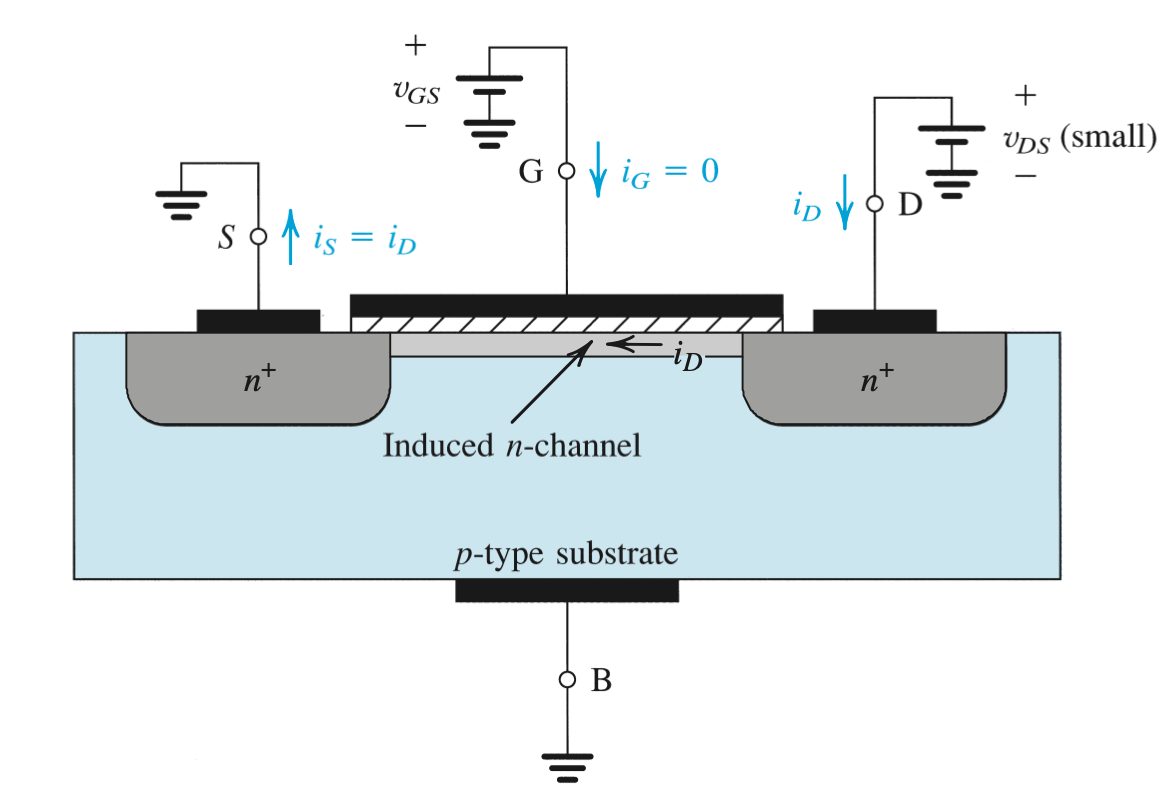
\includegraphics[scale=0.5]{figures/small_vds.png}}
        \textbf{Figure 1.3} NMOS with $v_{GS} > V_t$ and a small $v_{DS}$ applied.
        Of particular interest of calculating the current $i_D$ is the charge per
        unit channel length, which can be found as
    \end{center}
    \begin{align}
        \frac{|Q|}{unitChannelLenth} = C_{ox}Wv_{OV}
    \end{align}

    The voltage $v_{DS}$ establishes an electric field E across the length of the channel,
    \begin{align}
        |E| = \frac{v_{DS}}{L}
    \end{align}

    This electric field in turn causes the channel electrons to drift toward the drain with 
    a velocity given by
    \begin{align}
        \mu_n|E| = \mu_n\frac{v_{DS}}{L}
    \end{align}

    where $\mu_n$ is the mobility of the electrons at the surface of the channel. The value 
    of $i_D$ can now be found by multiplying the charge per unit channel length by the electron
    drift velocity.
    \begin{align}
        i_D = \left[(\mu_nC_{ox})\left(\frac{W}{L}\right)v_{OV}\right]v_{DS}
    \end{align}

    Thus, for small $v_{DS}$, the channel behaves as a linear resistance whose value is controlled 
    by the overdrive voltage $v_{OV}$ , which in turn is determined by $v_{GS}$
    \begin{align}
        i_D = \left[(\mu_nC_{ox})\left(\frac{W}{L}\right)(v_{GS}-V_t)\right]v_{DS}
    \end{align}

    The conductance $g_{DS}$ of the channel can be found by
    \begin{align}
        g_{DS} = (\mu_nC_{ox})\left(\frac{W}{L}\right)v_{OV}
    \end{align}

    Note that the \textit{\textbf{process transconductance}} parameter is given the symbol 
    $k_n' (A/V^2)$, where $n$ denotes n-channel
    \begin{align}
        k_n' = \mu_nC_{ox} 
    \end{align}

    The product of the process transconductance parameter $k_n'$ and the transistor aspect ratio
    $(W/L)$ is the MOSFET \textit{\textbf{transconductance parameter}} $k_n$,
    $$k_n = k_n'(W/L)$$
    We conclude this subsection by noting that with $v_{DS}$ kept small,the MOSFET behaves as a 
    linear resistance $r_{DS}$ whose value is controlled by the gate voltage $v_{GS}$,
    $$r_{DS} = 1/g_{DS}$$

    \subsection*{Operation as $v_{DS}$ is Increased (Saturation Region)}

    We next consider a situation where $v_{DS}$ is increased. $v_{GS}$ is held
    constant at a value greater than $V_t$; that is, the MOSFET will be 
    operated at a constant overdrive voltage $V_{OV}$. As we travel from source
    to drain, the voltage (measured relative to the source) increases from zero
    to $v_{DS}$. Thus the voltage between the gate and points along the channel 
    decreases from $v_{GS} = V_t + V_{OV}$ at the source end to $v_{GD} = v_{GS} 
    - v_{DS} = V_t + V_{OV} - v_{DS}$ at the drain end.

    Since the channel depth depends on the amount by which the voltage exceeds 
    $V_t$, we find that the channel is no longer uniform; being deepest at the 
    source end (where depth is proportional to $V_{OV}$) and shallowest at 
    the drain end (where depth is proportional to $V_{OV} - v_{DS}$).

    \begin{center}
        \centerline{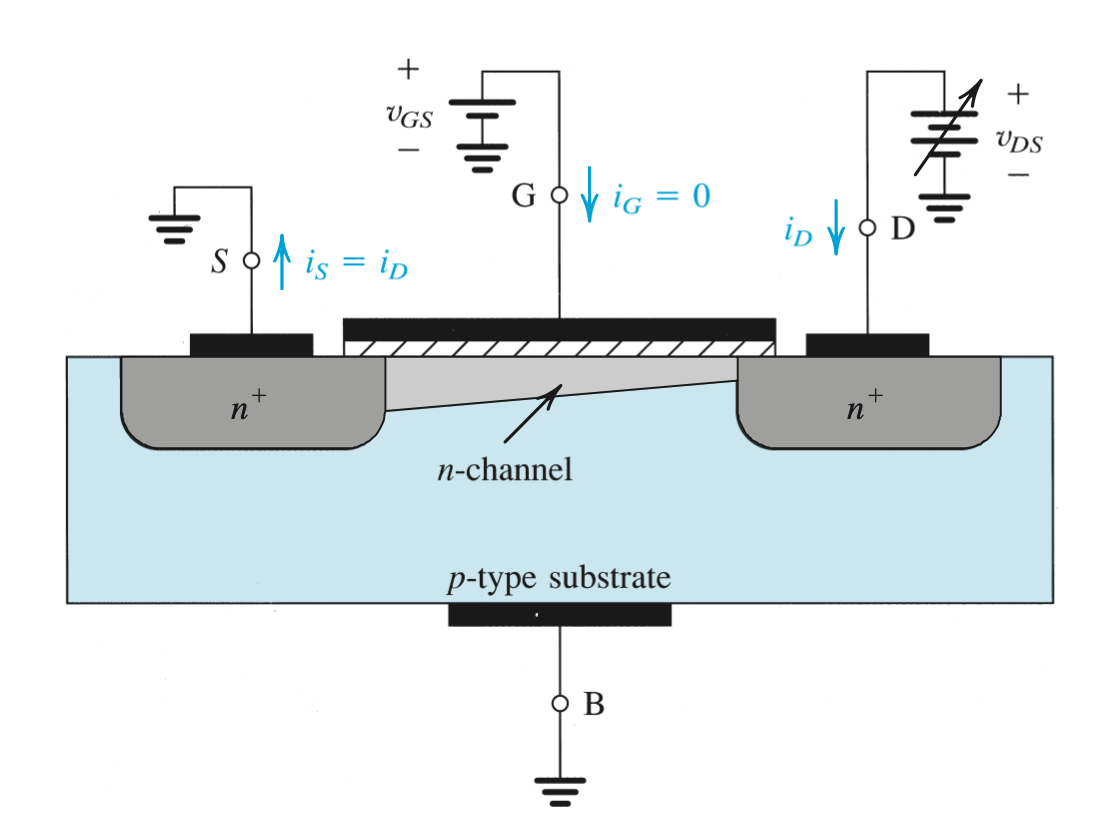
\includegraphics[scale=0.48]{figures/mosfet_induced2.png}}
        \textbf{Figure 1.4}
    \end{center}
    \begin{center}
        \centerline{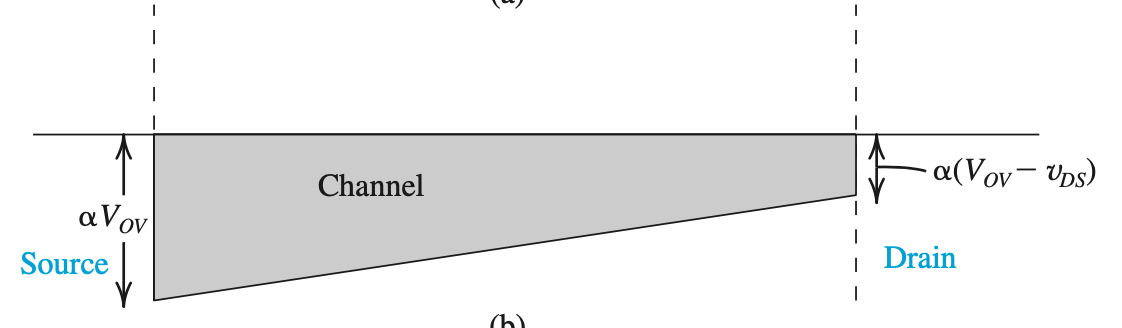
\includegraphics[scale=0.5]{figures/fig5.png}}
        \textbf{Figure 1.5}
    \end{center}
    \begin{center}
        \centerline{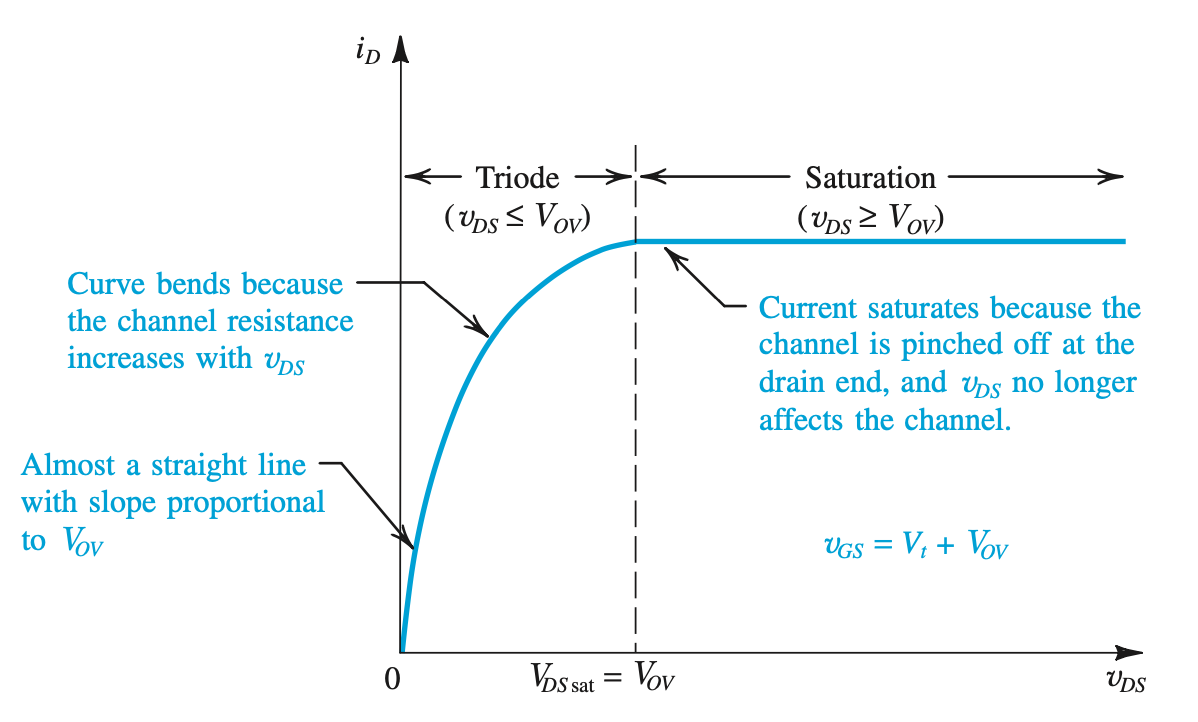
\includegraphics[scale=0.5]{figures/fig6.png}}
        \textbf{Figure 1.6}
    \end{center}

    As $v_{DS}$ is increased, the channel becomes more tapered and its resistance
    increases. Therefore the $i_D-v_{DS}$ curve does not continue in a straight 
    line, but bends as shown in \textbf{Figure 1.6}. Since the charge in the 
    tapered channel is proportional to the channel cross sectional shown in 
    \textbf{Figure 1.5}, the relationship between $i_D$ and $v_{DS}$ an be found
    as follows

    \begin{align}
        i_D = k_n'\left(\frac{W}{L}\right)\left(V_{OV} - \frac{1}{2}v_{DS}\right)v_{DS}
    \end{align} 

    This describes the \textit{\textbf{semiparabolic portion}} of the $i_D-v_{DS}$ curve.
    Notes that as $v_{DS}$ is reduced, we can neglect $\frac{1}{2}v_{DS}$ relative to 
    $V_{OV}$ and can be written as the equation shown in \textbf{(7)}.

    \subsection*{Operation for $v_{DS} \geq V_{OV}$ Channel Pinch-off and Current Saturation}

    The above description of operation assumed that even though the channel became
    tapered, it still had a finite (nonzero) depth at the drain end. This in turn is achieved 
    by keeping $v_{DS}$ sufficiently small that the voltage between the gate and the drain, 
    $v_{GD}$, exceeds $V_t$. \textbf{Figure 1.7} shows $v_{DS}$ reaching $V_{OV}$ and $v-{GD}$ 
    corrispondingly reaching $V_t$. The zero depth of the channel gives rise to the term 
    \textit{\textbf{channel pinch-off}}. Increasing $v_{DS}$ beyond this point 
    $(i.e., v_{DS} > V_{OV})$, has no effect on the channel shape and charge.

    \begin{center}
        \centerline{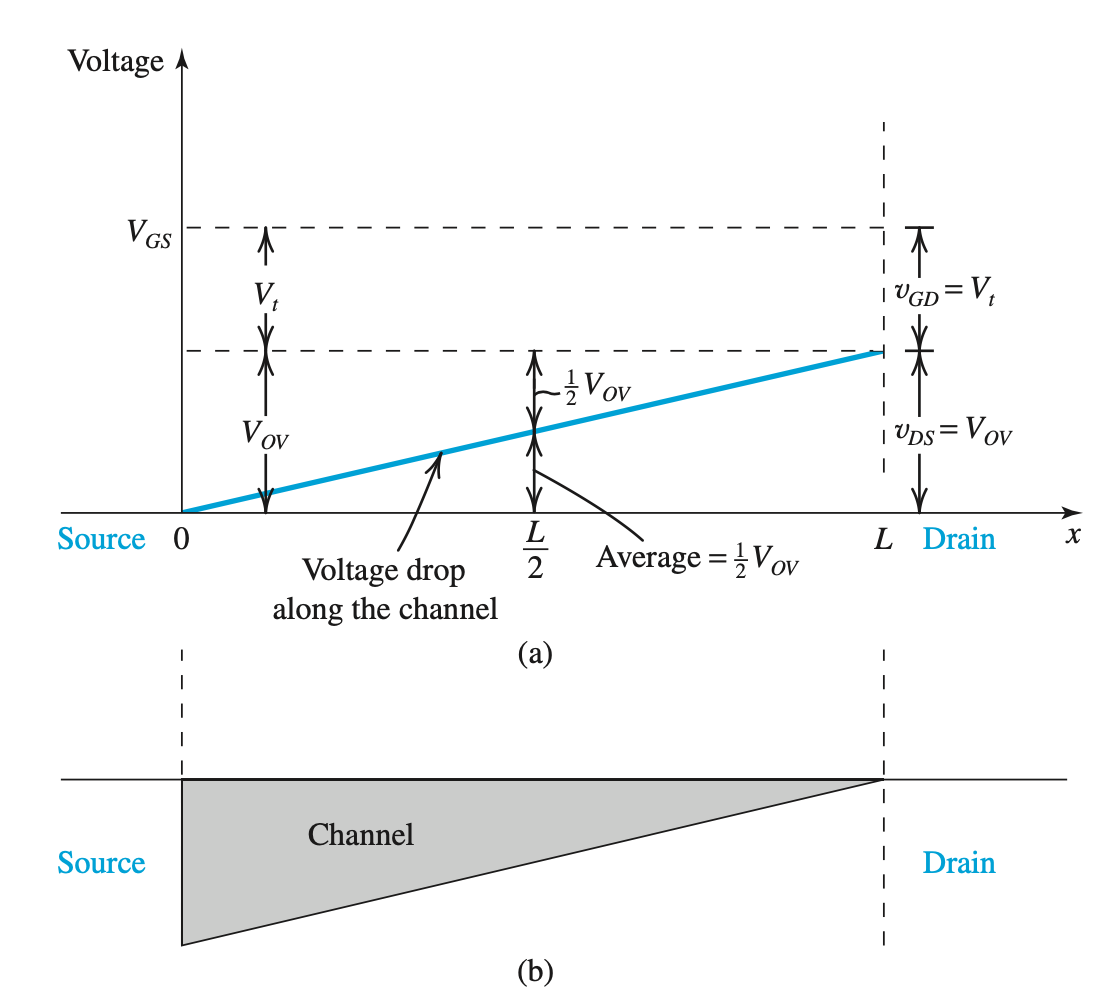
\includegraphics[scale=0.6]{figures/fig7.png}}
        \textbf{Figure 1.7}
    \end{center}

    The drain current thus \textit{\textbf{saturates}} at the value found by substituting 
    $v_{DS} = V_{OV}$

    \begin{align}
        i_D = \frac{1}{2}k_n'\left(\frac{W}{L}\right)V^2_{OV}
    \end{align}

    *$V_{OV}$ can be replaced by $v_{OV}$ and $v_{OV}$ by $(v_{GS}-V_t)$\\[\baselineskip]
    The MOSFET is then said to have entered the \textit{\textbf{saturation region}}. The voltage 
    $v_{DS}$ at which saturation occurs is denoted $V_{DSsat}$

    \begin{align}
        V_{DSsat} = V_{OV} = V_{GS} - V_t
    \end{align}

    The channel pinch off does \textit{not} mean channel blockage. Current continues to flow
    through the pinched-off channel and the electrons that reach the drain end are 
    accelerated through depletion region. Any increase in $v_{DS}$ above $V_{DSsat}$ appears as 
    a voltage drop across the depletion region.  

    \subsection*{Finite Output Resistance in Saturation}

    \begin{center}
        \centerline{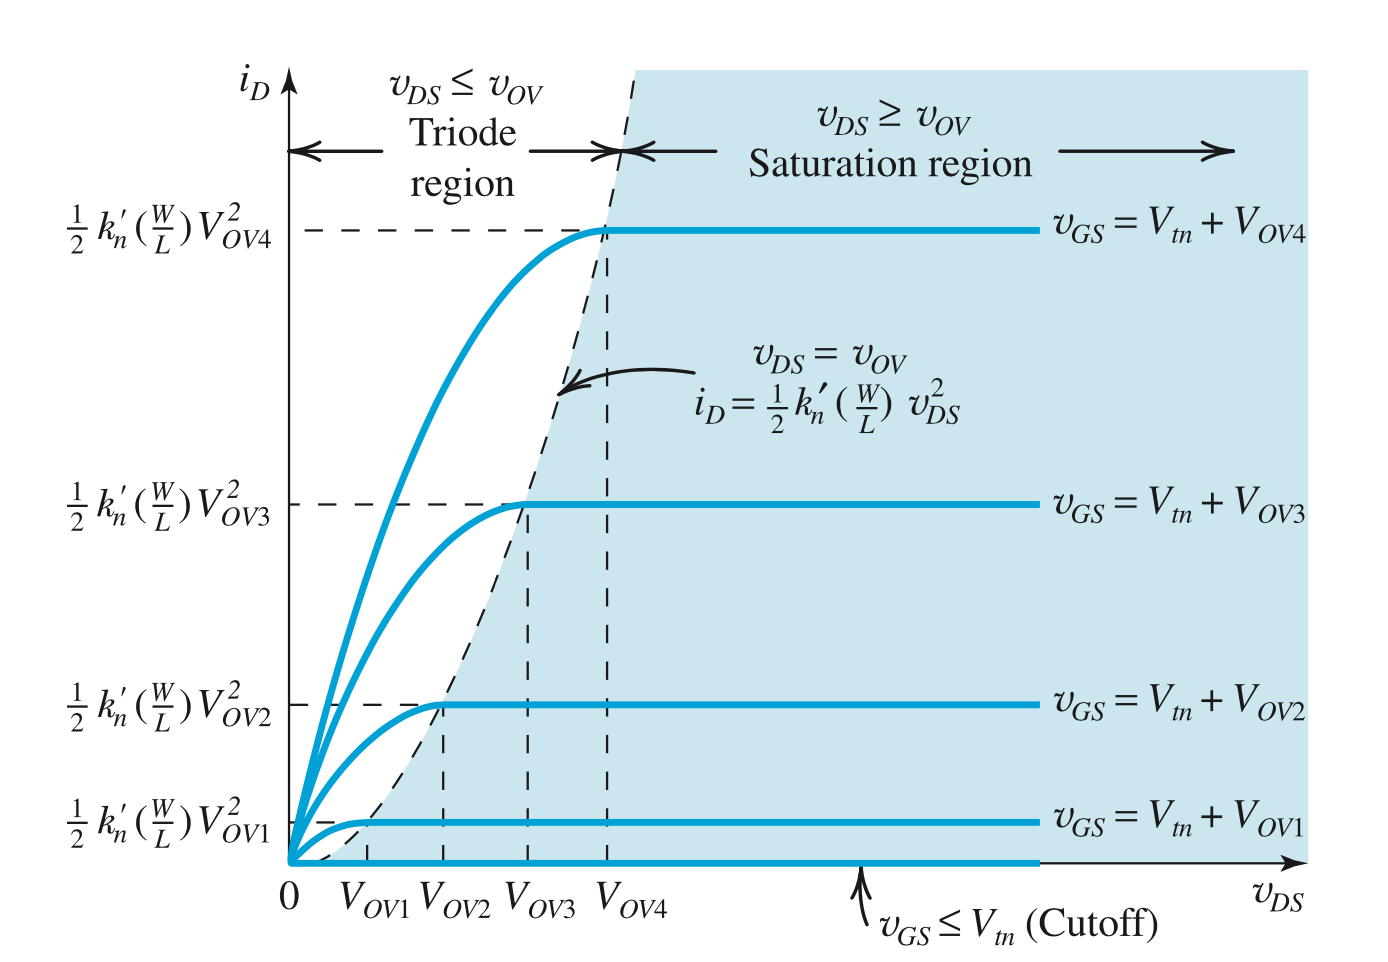
\includegraphics[scale=0.5]{figures/fig14.png}}
        \textbf{Figure 1.8} $i_D-v_{DS}$ characteristics of enhancement type NMOS transistor.
    \end{center}

    Figure 1.8 indicates that in saturation, $i_D$, is independent of $v_{DS}$, thus a change in 
    $v_{DS}$ in the drain to source voltage causes no change in $i_D$ so the resistance looking 
    into the drain of a saturated MOSFET is infinite. However, there is in fact an effect from
    increasing $v_{DS}$ beyond $v_OV$ which is that the channel pinch off point moves slightly 
    away from the drain and towards the source. The channel length is in effect reduced from 
    $L$ to $L-\Delta L$, a phenomenon known as \textbf{channel-length modulation}. 

    \begin{center}
        \centerline{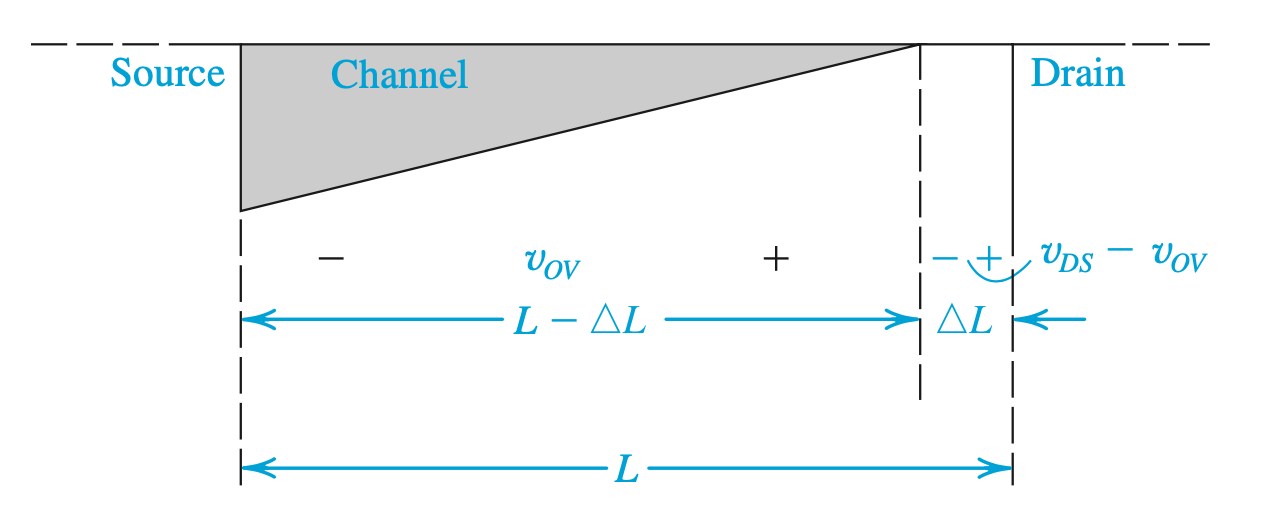
\includegraphics[scale=0.5]{figures/fig16.png}}
        \textbf{Figure 1.9}
    \end{center}
    
    This effect can be accounted for by

    \begin{align}
        i_D = \frac{1}{2}k_n'\left(\frac{W}{L}\right)(v_{GS}-V_{tn})^2(1+\lambda v_{DS})
    \end{align}

    \subsection*{P-Channel MOSFET}

    \begin{center}
        \centerline{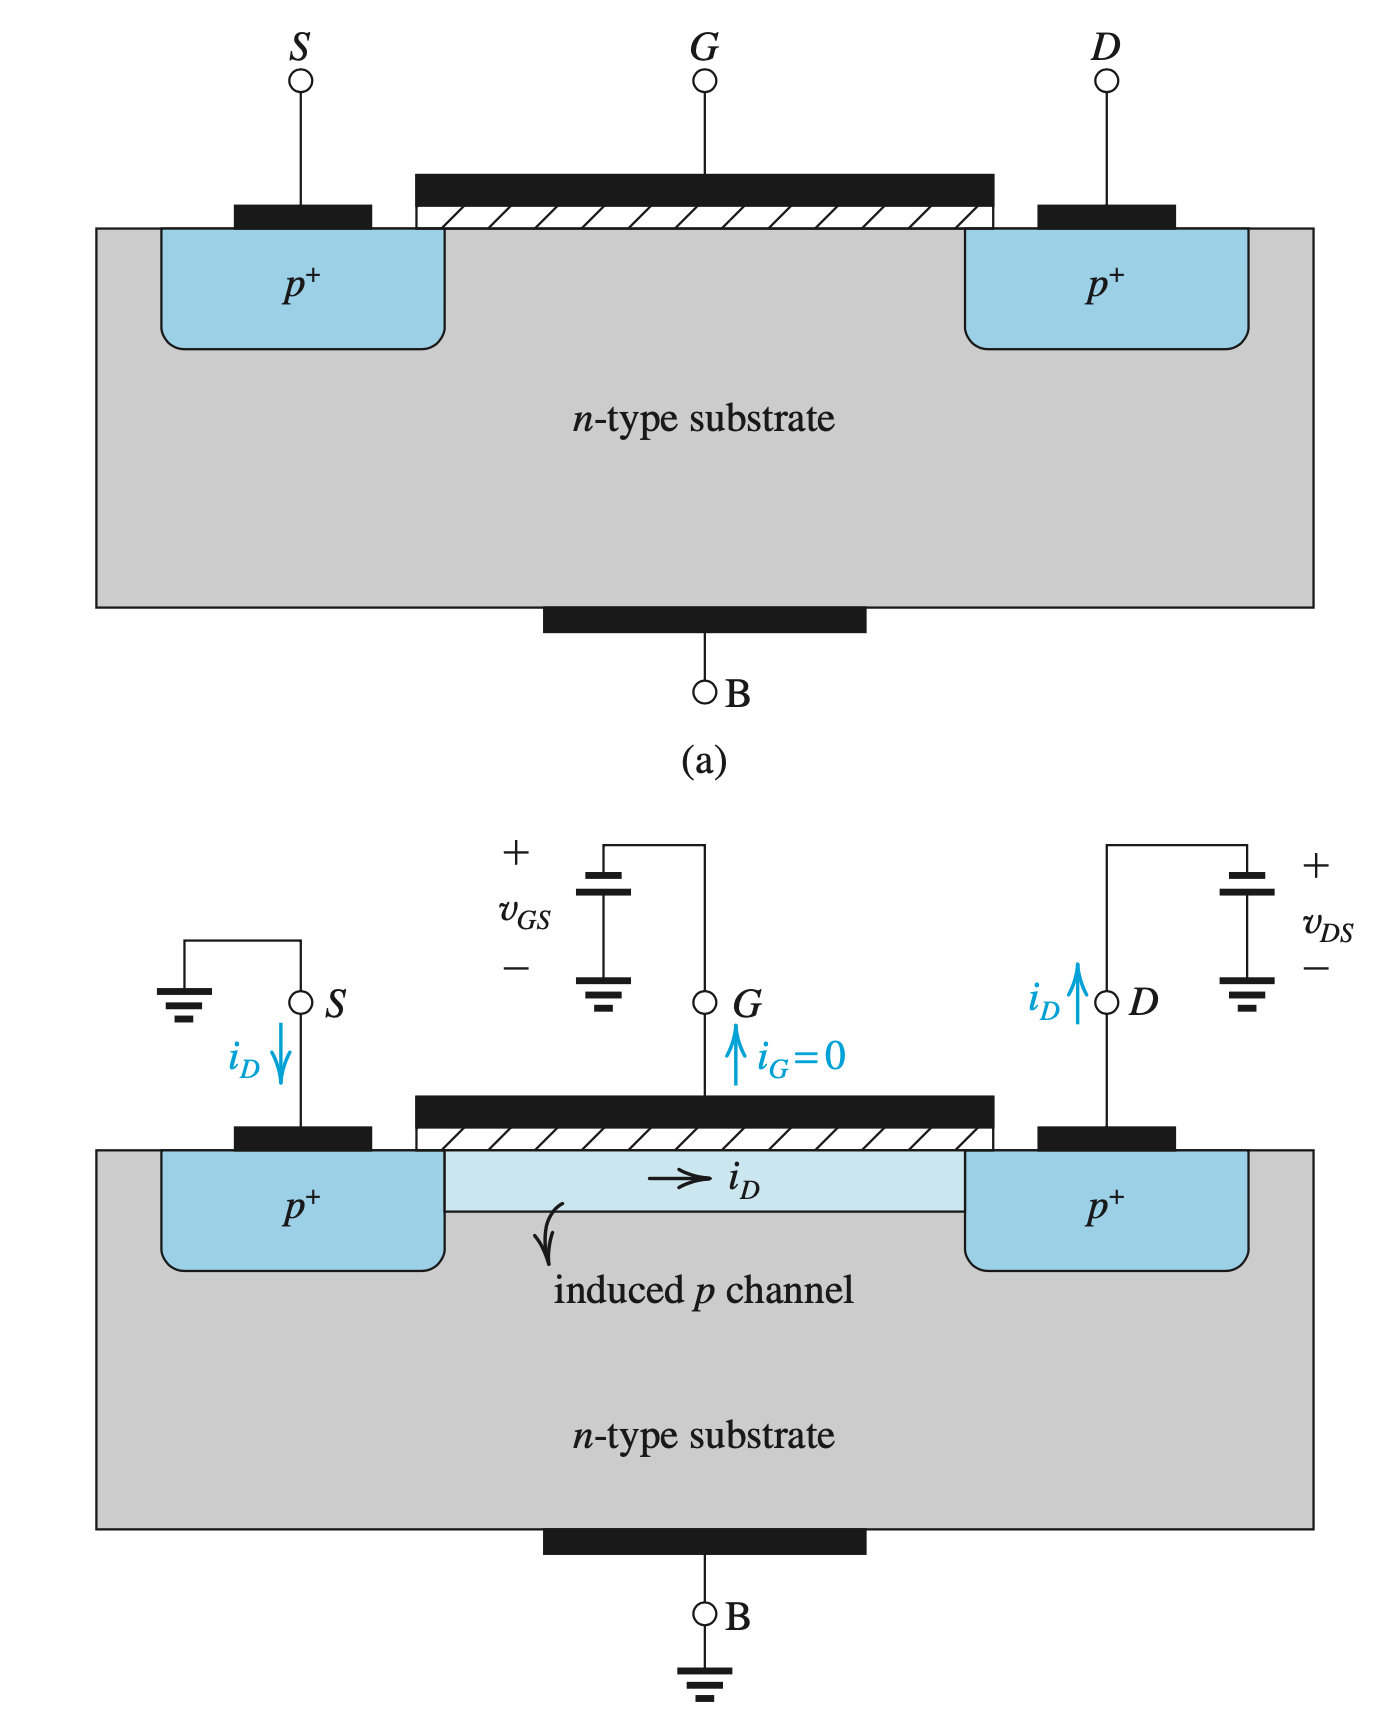
\includegraphics[scale=0.5]{figures/fig13.png}}
        \textbf{Figure 1.10} P-Channel MOSFET.
    \end{center}
    
    To induce current flow between source and drain, a negative voltage is applied to the gate. Once
    the magnitude of the negative $v_{GS}$ is beyond that of the threshold voltage $V_{tp}$, the 
    p-channel is established.

    $$v_{GS} \leq V_{tp}$$
    or
    $$|v_{GS}| > |V_{tp}|$$

    To cause a current $i_D$ to flow through the channel, a negative voltage $v_{DS}$ is applied to 
    the drain. The current $i_D$ is carried by holes and flows through the channel from source to drain.

    \subsection*{Implications of Scaling}

    \begin{center}
        \centerline{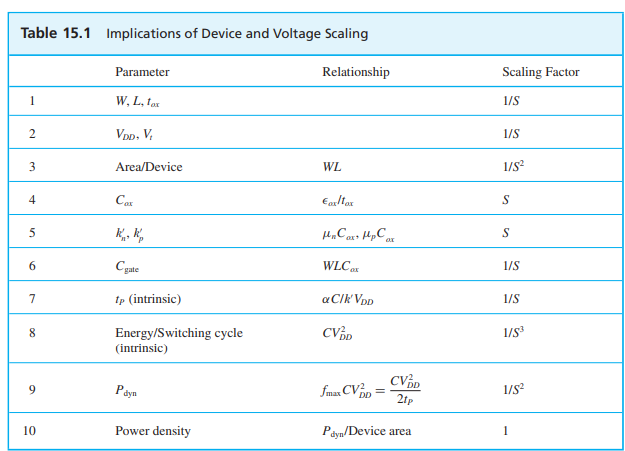
\includegraphics[scale=1]{figures/scaling.png}}
    \end{center}
    \subsection*{Summary}

    \begin{center}
        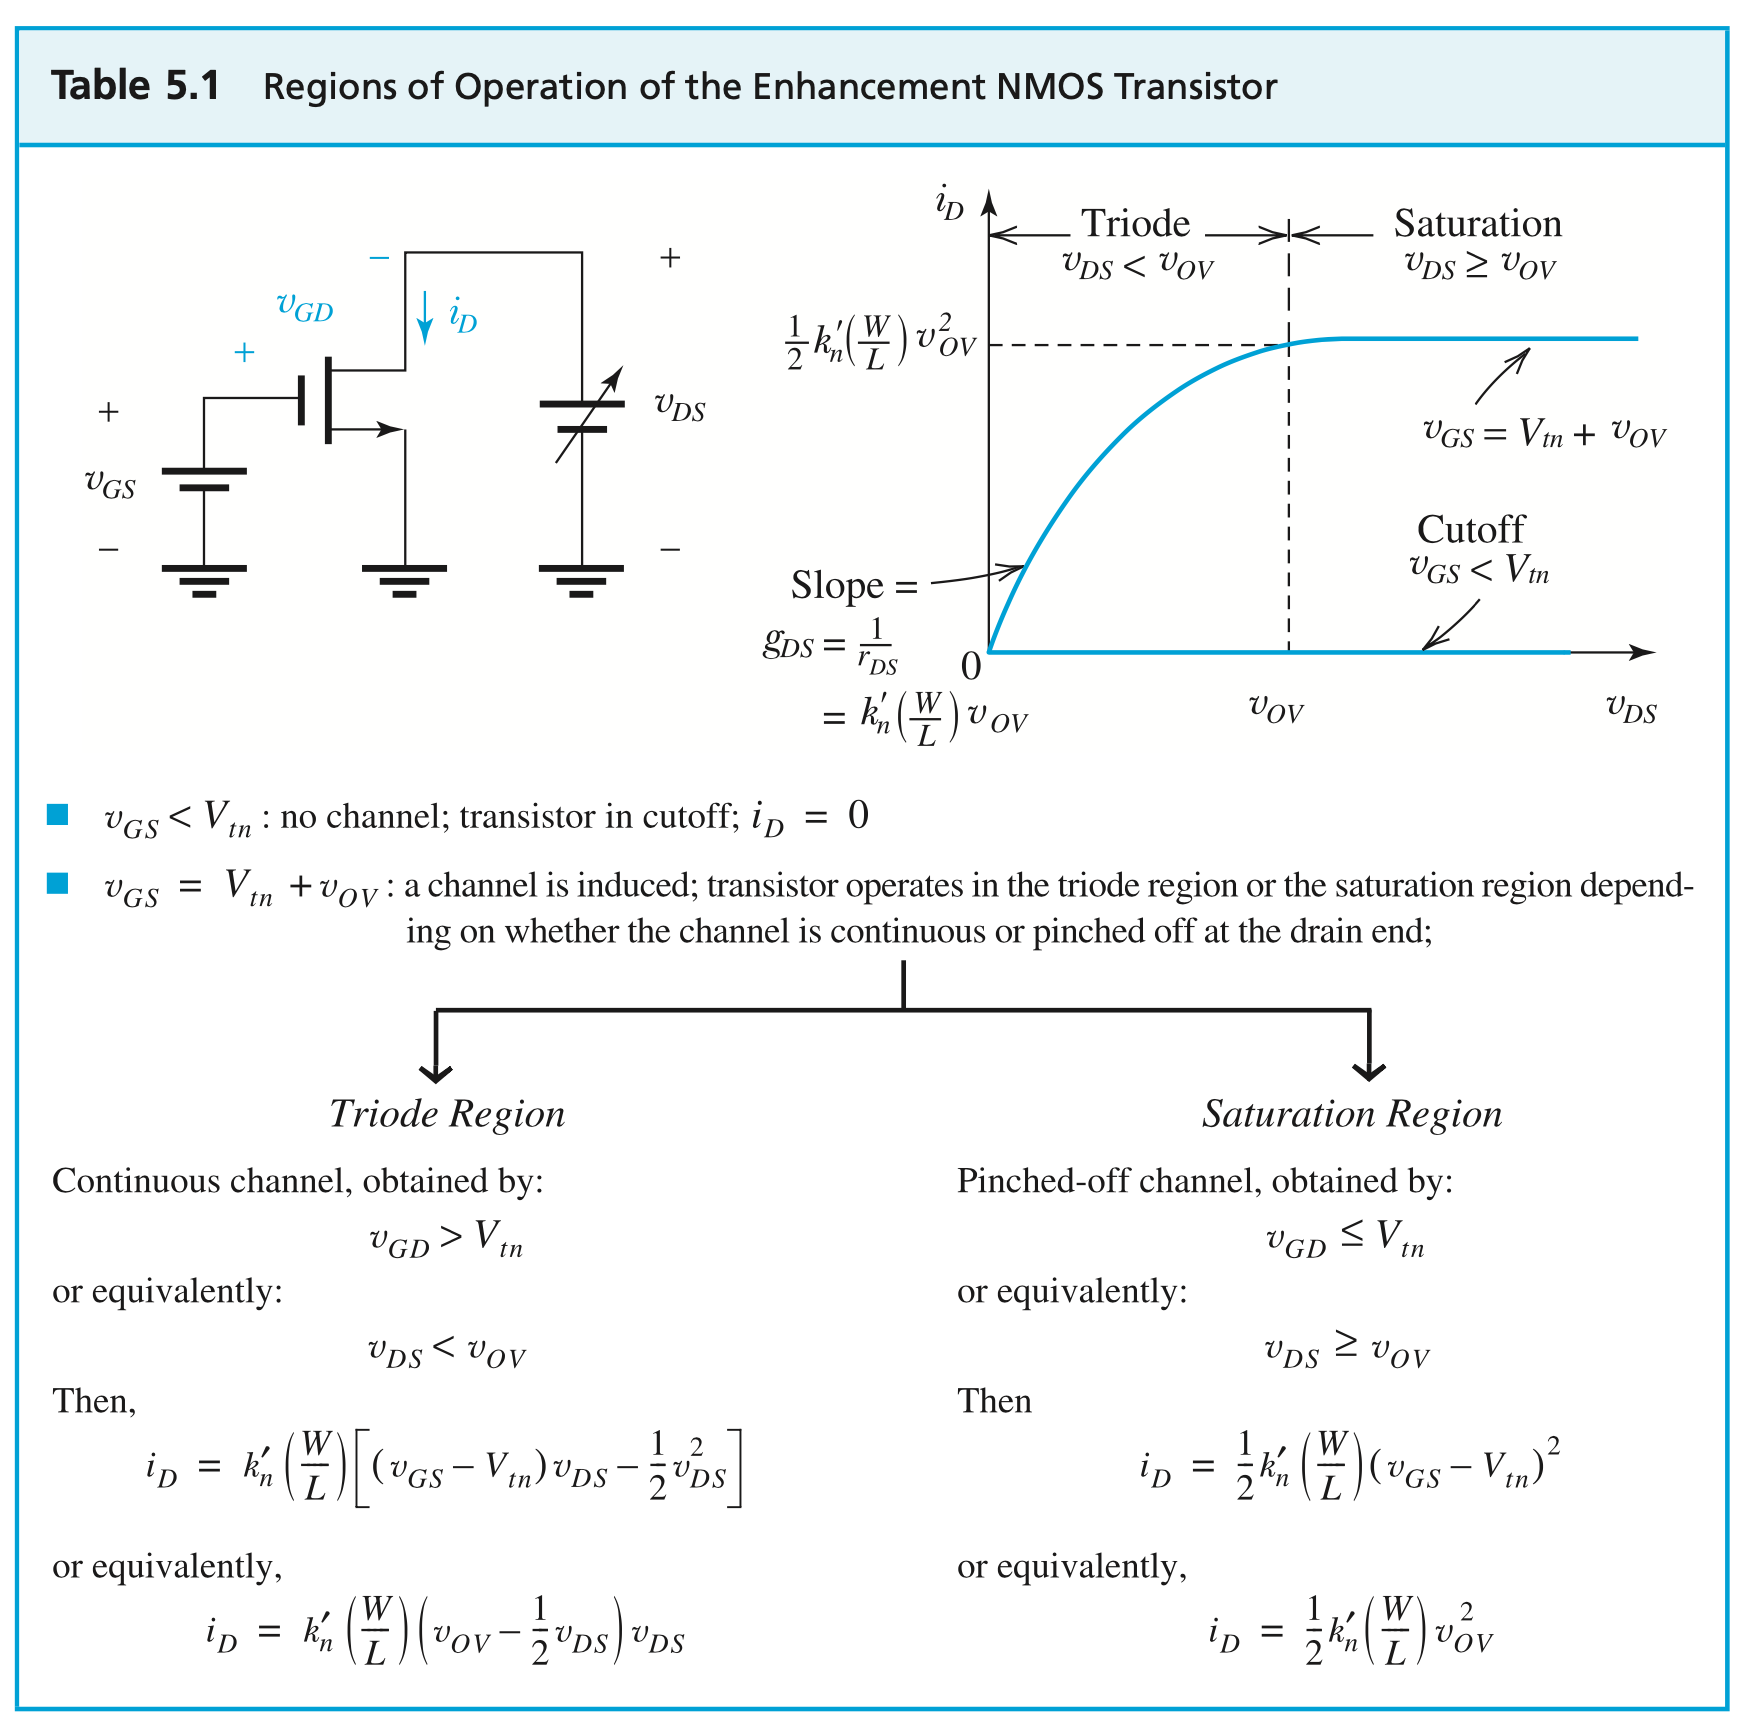
\includegraphics[scale=0.5]{figures/fig18.png}
        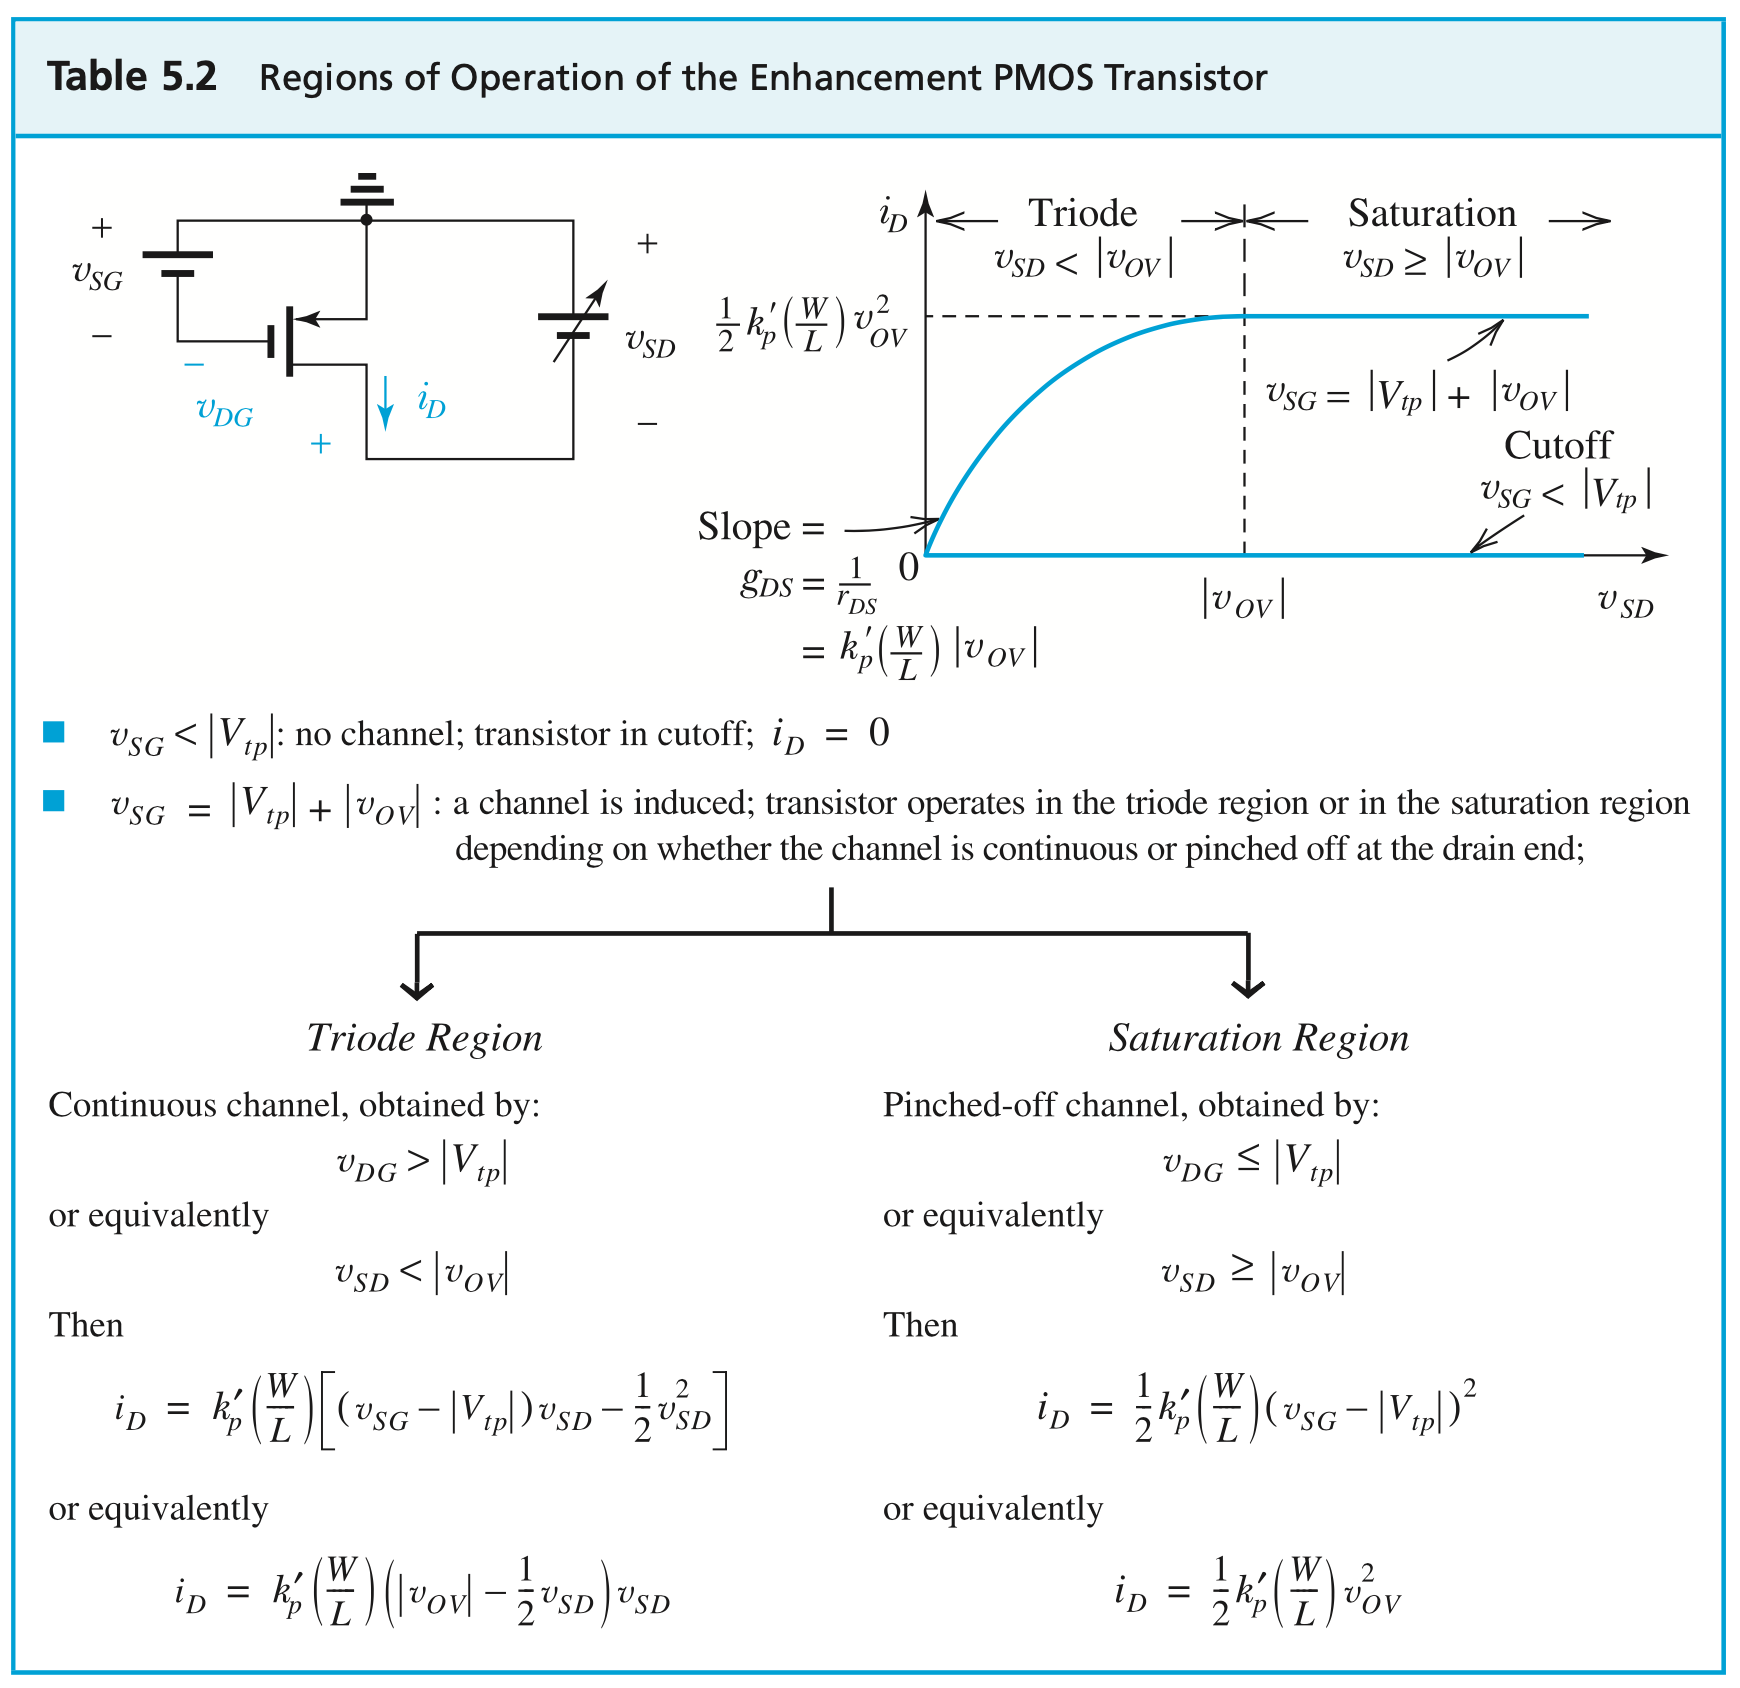
\includegraphics[scale=0.5]{figures/fig17.png}
    \end{center}

    \subsection*{Short and Long Channel Model}

    \section{CMOS Logic-Gate Circuits}

    In this section we consider the synthesis of CMOS circuits that realize combinational logic 
    functions. In combinational circuits, the output at any time is a function only of the values 
    of input signals at that time. Thus, these circuits do not have memory and do not employ 
    feedback. Combinational circuits are used in large quantities in every digital system.
    
    \subsection*{Switch Level transistor Model}

    CMOS digital circuits utilize NMOS and PMOS transistors operating as \textit{switches}.
    An NMOS transistor behaves as a closed switch, exhibiting a very small resistance ($R_{on}$ or 
    $r_{DS}$) between its drain and source when its gate voltage is “high,” usually at the power 
    supply level $V_{DD}$, which represents a logic 1. Conversely, when the gate voltage is “low” 
    (i.e., at or close to ground voltage), which represents a logic 0, the transistor is cut off, 
    thus conducting zero current and acting as an open switch.
    
    \begin{center}
        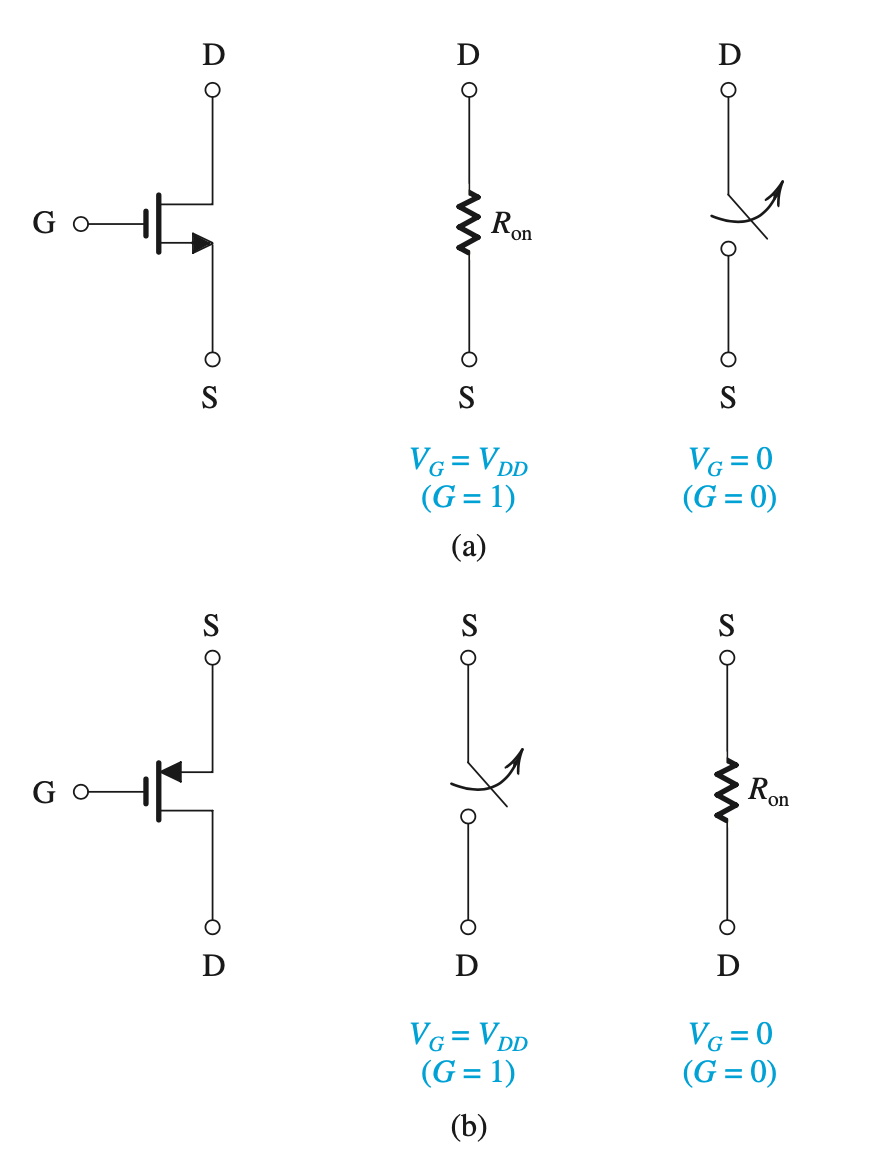
\includegraphics[scale=0.6]{figures/fig8.png}
    \end{center}
    \textbf{Figure 2.1} (a) NMOS and (b) PMOS transistors as a switch.
    
    \subsection*{CMOS Inverter}

    \begin{center}
        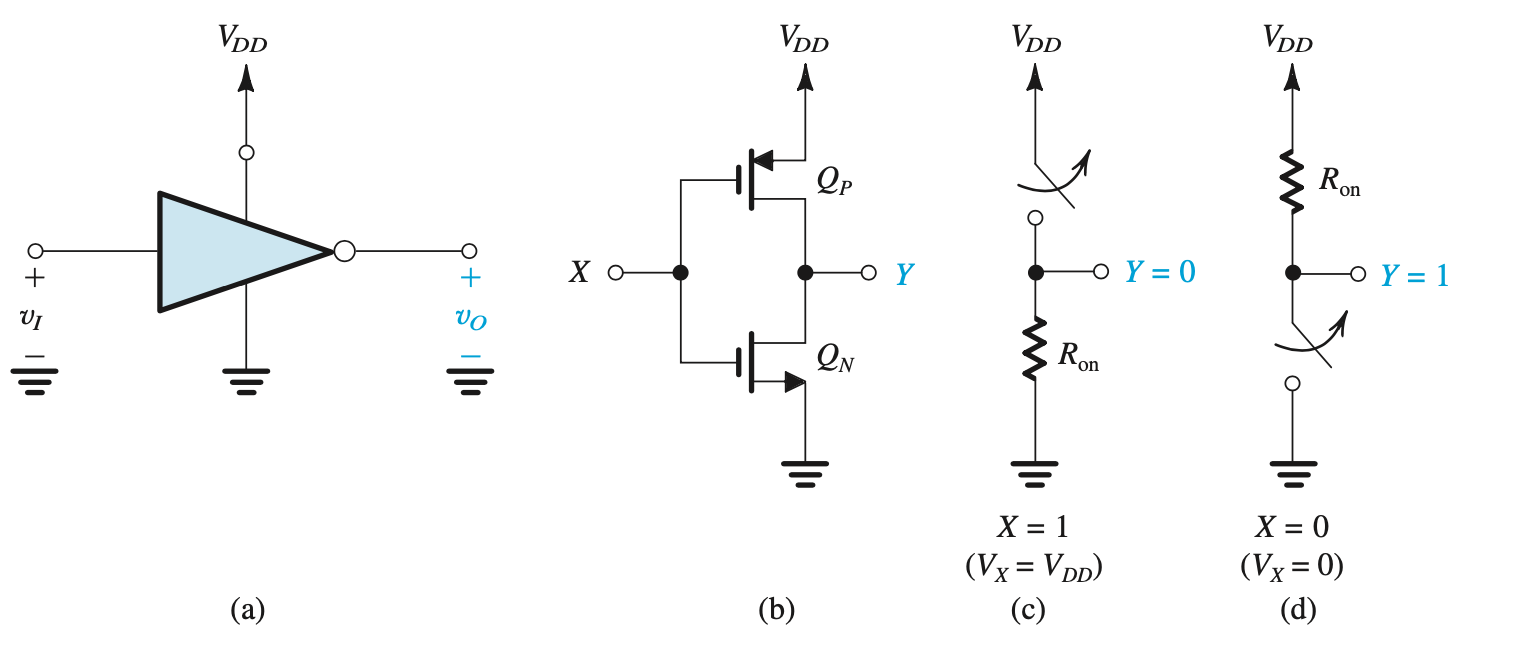
\includegraphics[scale=0.5]{figures/fig9.png}
    \end{center}
    \textbf{Figure 2.2} The inverted operated from a power supply $V_{DD}$ is shown in (a). Its 
    CMOS circuit implementation is shown in (b). (c) and (d) shows when the input $V_x = V_{DD}$ 
    and $V_x = 0$ respectively.

    \subsection*{Inverter Circuit Operation}

    We first consider the two extreme cases: when $v_I$ is at logic-0 level, which is 0V, and 
    when $v_I$ is at logic-1 level, which is $V_{DD}$ volts.

    \begin{center}
        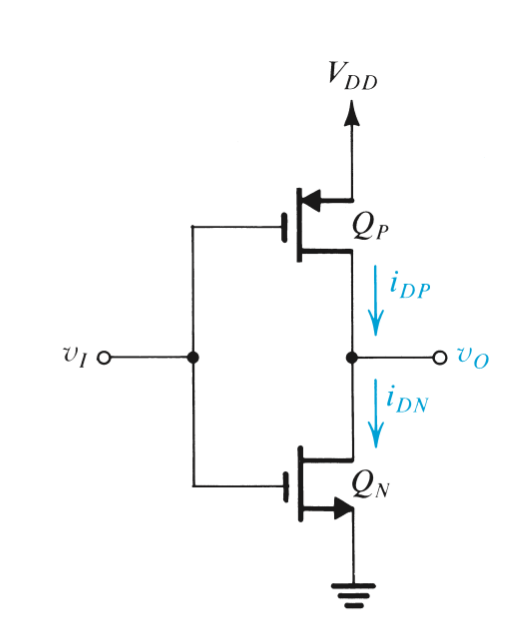
\includegraphics[scale=0.6]{figures/fig10.png}
    \end{center}
    \textbf{Figure 2.3} CMOS Inverter

    \begin{center}
        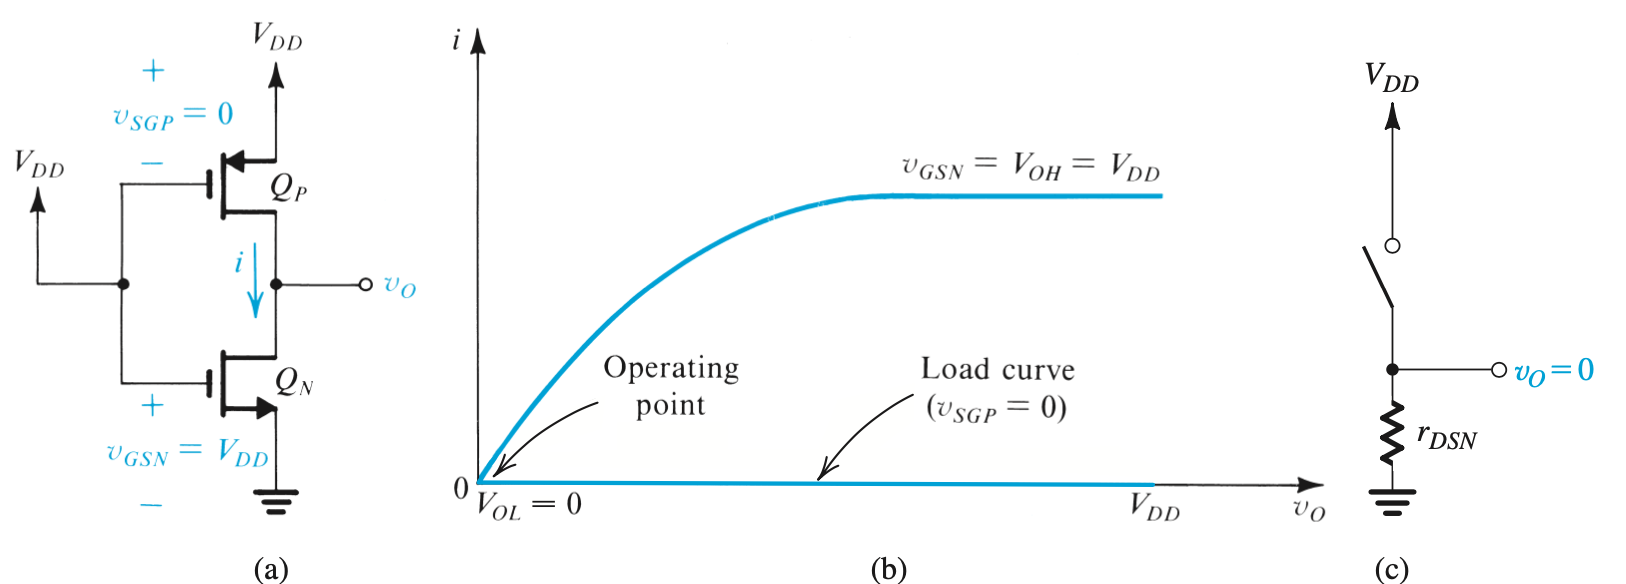
\includegraphics[scale=0.45]{figures/fig11.png}
    \end{center}

    \textbf{Figure 2.4} CMNOS Inverter when $v_I$ is high.\\[\baselineskip]
    Illustrated is the case when $v_I = V_{DD}$, showing the $i_D-v_{DS}$ characteristic curve 
    for $Q_N$ with $v_{GSN} = V_{DD}$. (Note that $i_D = i$ and $v_{DSN} = v_O$). Superimposed 
    on the $Q_N$ characteristic curve is the load curve, which is the $i_D-v_{SD}$ curve of $Q_P$
    for the case $v_{SGP} = 0 V$. Since $v_{SGP} < |V_t|$, the load curve will be a horizontal 
    straight line at zero current level. The operating point will be at the intersection of the 
    two curves, where we note that the output voltage is zero and the current through the two 
    devices is also zero. This means that the power dissipation in the circuit is zero. Note, 
    however, that although $Q_N$ is operating at zero current and zero drain-source voltage 
    (i.e., at the origin of the $i_D-v_{DS}$ plane), the operating point is on a steep segment 
    of the $i_D-v_{DS}$ characteristic curve. Thus $Q_N$ provides a low-resistance path between 
    the output terminal and ground, with the resistance obtained using
    \begin{align}
        r_{DSN} = \frac{1}{[k_n'(\frac{W}{L})_n(V_{DD}-V_{tn})]}  
    \end{align}

    \begin{center}
        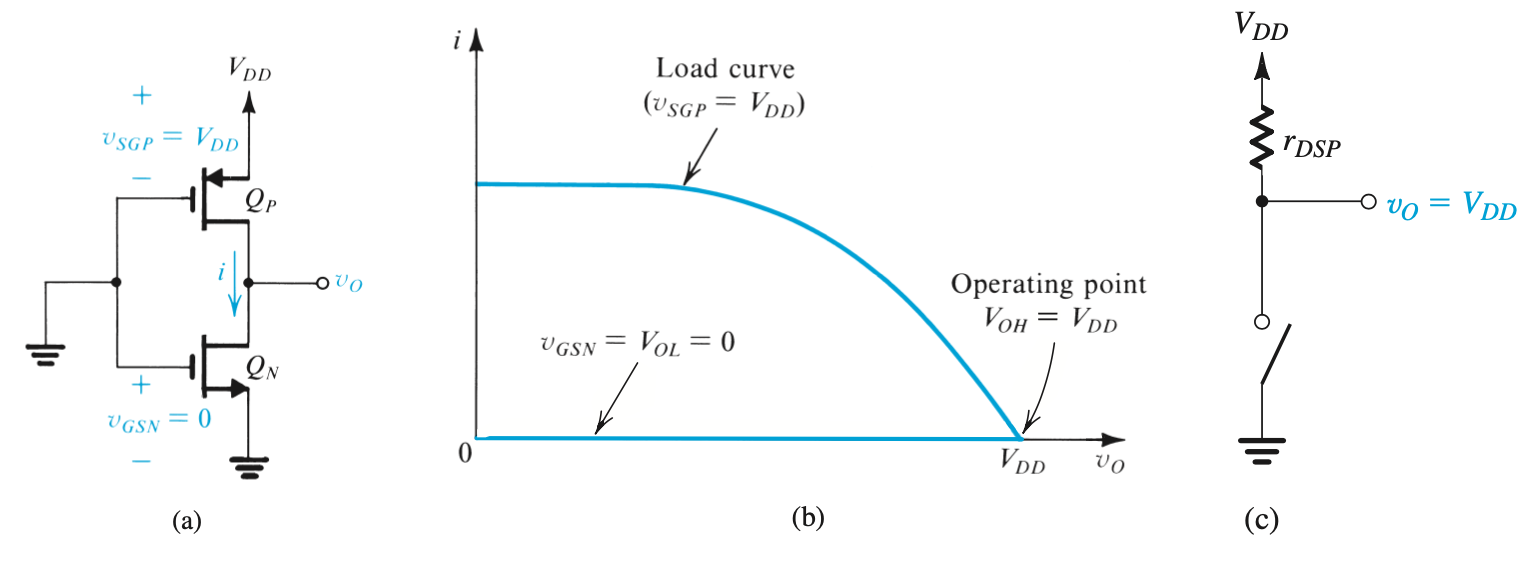
\includegraphics[scale=0.45]{figures/fig12.png}
    \end{center}
    \textbf{Figure 2.5} CMOS inverter when $v_I$ is low.\\
    
    \begin{align}
        r_{DSP} = \frac{1}{\left[k_p'(\frac{W}{L})_p(V_{DD}-|V_{tp}|)\right]}
    \end{align}

    \subsection*{Ideal Inverter Voltage Transfer Characteristics}

    \begin{center}
        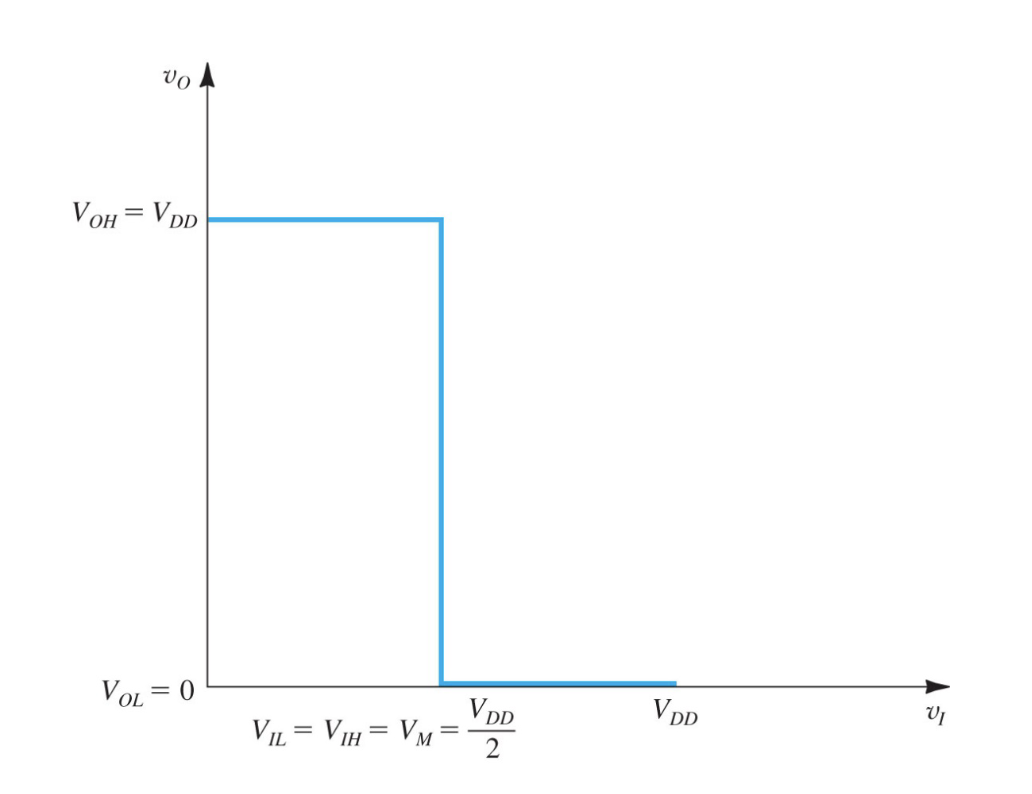
\includegraphics[scale=0.75]{figures/s2.png}
    \end{center}

    \begin{itemize}
        \item maximum output signal swing
        \begin{itemize}
            \item $V_{OH} = V_{DD}$
            \item $V_{OL} = O$
        \end{itemize}
        \item maximized noise margins
        \item transition region has zero width
    \end{itemize}

    \begin{center}
        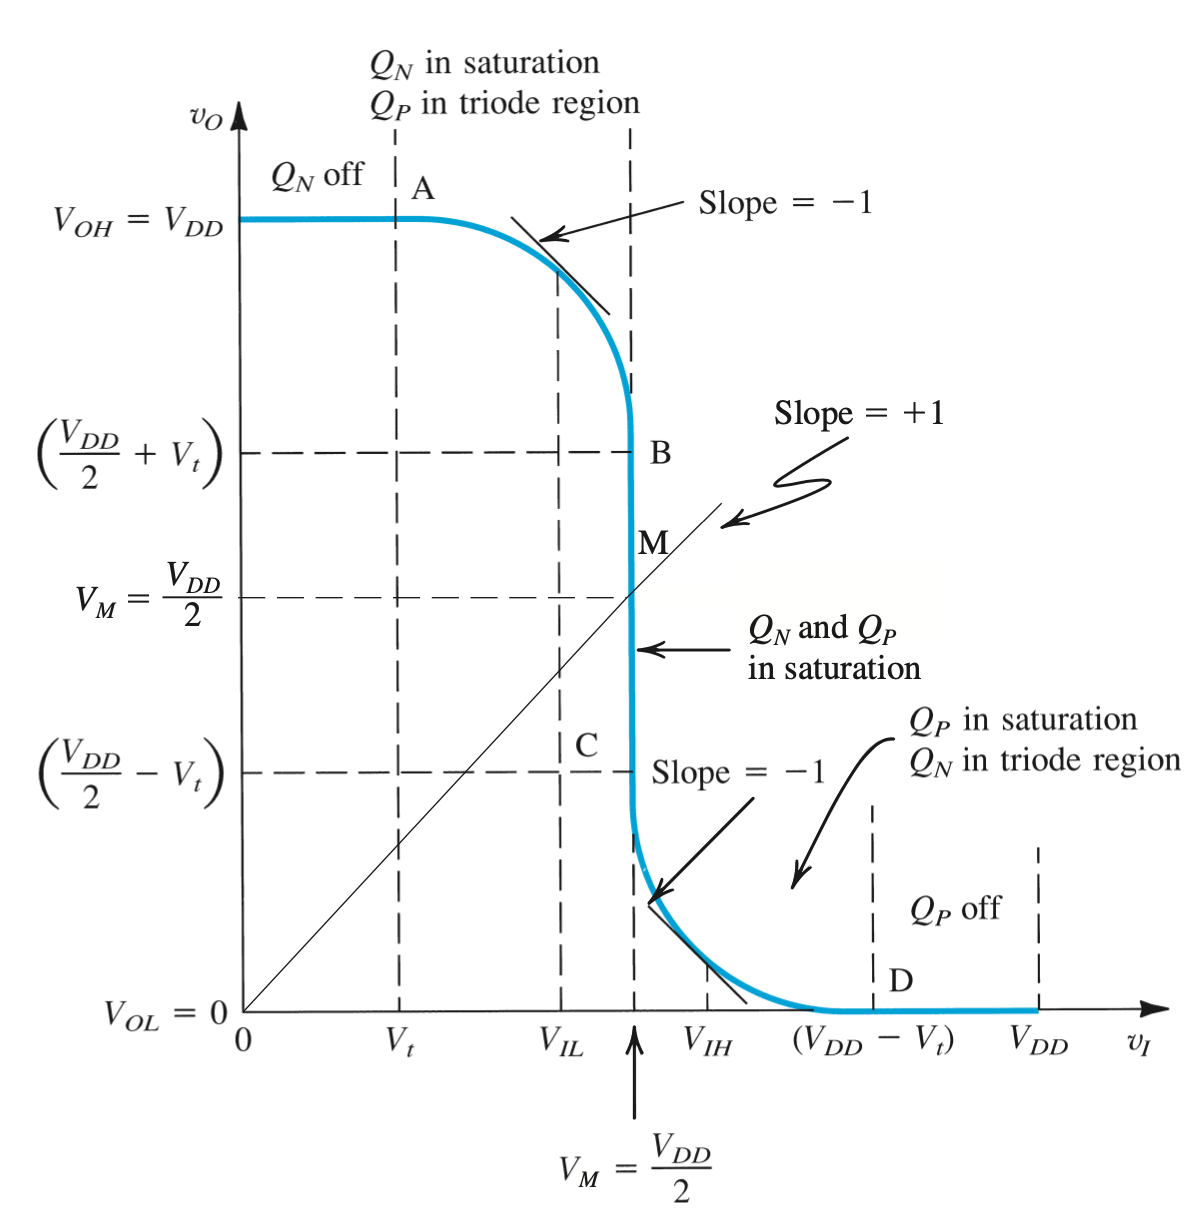
\includegraphics[scale=0.5]{figures/fig19.png}
    \end{center}

    for $v_O \leq v_I - V_{tn}$
    \begin{align}
        i_{DN} = k_n'\left(\frac{W}{L}\right)_n\left[(v_I - V_{tn})v_O-\frac{1}{2}v_O^2\right]
    \end{align}
    and for $v_O \geq v_I - V_{tn}$
    \begin{align}
        i_{DN} = k_n'\left(\frac{W}{L}\right)_n(v_I - V_{tn})^2
    \end{align}
    for $v_O \geq v_I +|V_{tp}|$
    \begin{align}
        i_{DP} = k_p'\left(\frac{W}{L}\right)_p\left[(V_{DD}-v_I-|V_{tp}|)(V_{DD}-v_O)-\frac{1}{2}(V_{DD}-v_O)^2\right]
    \end{align}
    and for $v_O \leq v_I +|V_{tp}|$
    \begin{align}
        i_{DP} = \frac{1}{2}k_p'\left(\frac{W}{L}\right)_p(V_DD-v_I-|V_{tp}|)^2
    \end{align}

    \subsection*{Inverter VTC}

    \begin{center}
        \centerline{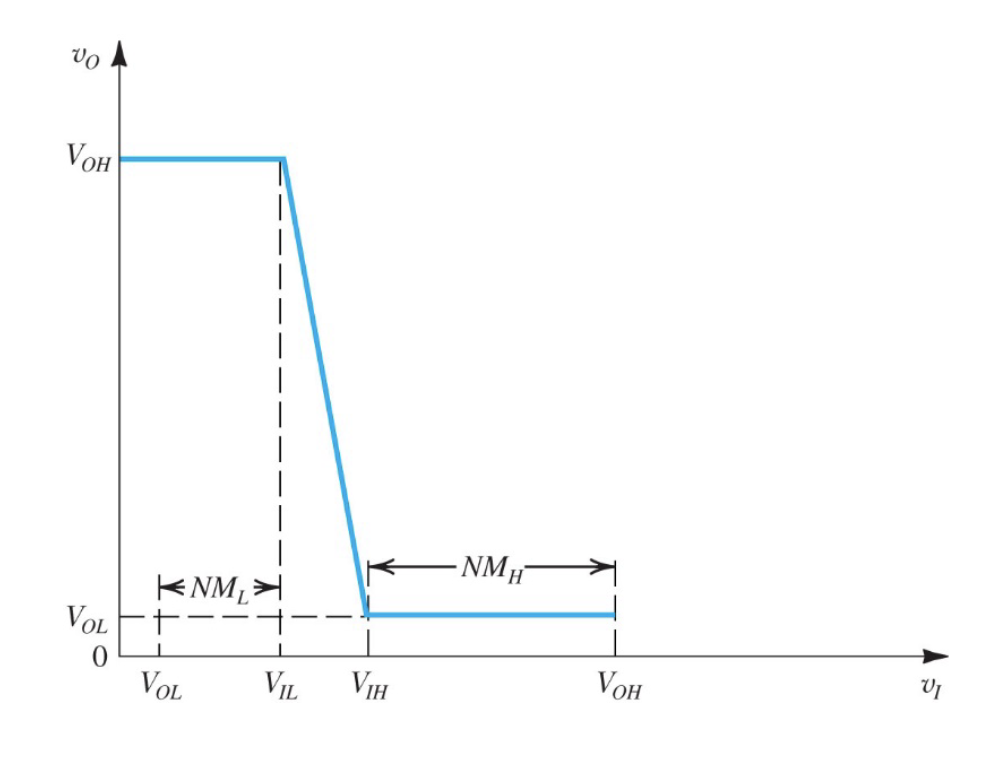
\includegraphics[scale=0.6]{figures/s3.png}}
    \end{center}
    
    * Straight line VTC approx.

    $V_{OH} \leq V_{DD}$
    $V_{OL} \geq 0$
    *finite transition region: $V_{IH} - V_{IL}$
    $V_{OH}$ does not depend on $v_I$ as long as $v_I \leq v_{IL}$
    $V_{OL}$ does not depend on $v_I$ as long as $v_i \geq V_{IH}$
    *looking to maximize noise margins

    \subsection*{Inverter Noise Margins}

    $$NM_L = V_{IL} - V_{OL}$$
    L: low
    $$NM_H = V_{OH} - V_{IH}$$

    \subsection*{Typical Inverter VTC}

    $V_{OL}$: output low
    $V_{OH}$: output high
    $V_{IL}$: max input interpreted as a logic 0
    $V_{IH}$: max input interpreted as a logic 1

    \subsection*{Ring Oscillators}

    Consists of an odd number of inverters in a circular chain
    Can be used to determine propagation delay or as a clock signal
    $f = \frac{1}{2Ntp}$ where n is the number of inverters
    $f = \frac{1}{N(t_{PLH} + t_{PHL})}$ if $t_{PLH}$ not equal to $t_{PHL}$

    \subsection*{MOSFET Amplifier as an Inverter}

    When $v_I = 0$, $v_O = V_{DD}$ since the transistor is off

    When $v_I = V_{DD}, v_O =$
    in triode region and will be modeled as a resistor

    *For $v_I \leq V_t$, the NMOS is \textbf{off}
    $i_D = 0$ and $v_O = V_{OH} - V_{DD}$

    *When $v_I$ exceeds $V_t$, the MOSFET turns on an initially is in the \textit{saturation region} (B to C)
    $$i_D = \frac{1}{2}K_N(v_I - V_t)^2$$
    $$v_O = V_{DD} - i_dR_d = V_{DD} - \frac{1}{2}K_nR_D(v_I - V_t)^2$$

    *Beyond point C, the transistor is in the triode region
    $$i_D = K_n[(v_I - V_t)v_O - \frac{1}{2}(v_O)^2]$$
    $$v_O = V_{DD} - i_DR_D = V_{DD} - K_NR_D[(v_I - V_t)v_O - \frac{1}{2}(v_O)^2]$$

    \section{CMOS Inverter VTC}

    Considering any possible input $v_I$, from 0V to $V_{DD}$, we will look at the potential operating regions
    of the NMOS and PMOS transistors. \textit{\textbf{The following assumes that the NMOS and PMOS transistors 
    are matched (assuming equal length), so:}}
    \begin{align*}
        k_n'\left(\frac{W}{L}\right)_n = k_p'\left(\frac{W}{L}\right)_p
    \end{align*}
    or
    \begin{align*}
        \frac{W_p}{W_n} = \frac{\mu_n}{\mu_p}
    \end{align*}

    \subsection*{Transistor Regions of Operation}

    \begin{center}
        \centerline{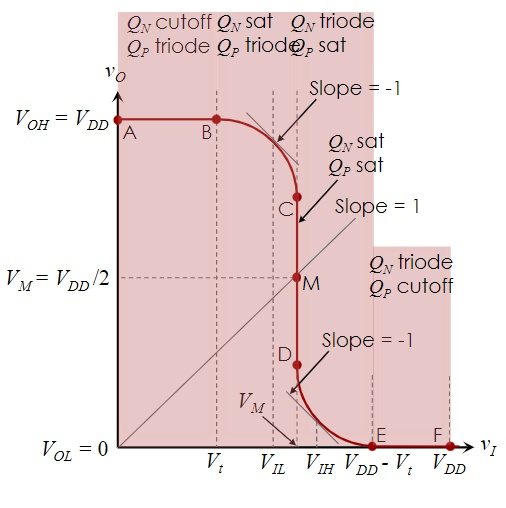
\includegraphics[scale=0.5]{figures/CMOS_VTC.jpg}}
    \end{center}
    
    \end{document}